\section{Online machine learning and reinforcement learning}
    Online machine learning, also known as incremental or sequential learning, is a type of machine learning where models are learned and improved over time as new data becomes available. Rather than training a model on a fixed dataset all at once, online machine learning allows the model to adapt and evolve in response to changing conditions.

    One of the main benefits of online machine learning is that it can reduce the amount of time and computational resources required for training and updating a model. Rather than starting from scratch each time new data is added, the model can build on previous knowledge, leading to more efficient learning.


\section{Electronic market making}
    We need to define the market making problem in the market. As it was stated in \cite{Cartea2015} and \cite{Bouchaud2018},
    the objective of the electronic market is to match the buy and sell orders 
    of the market participants. In practice we can divide all orders to 
    the two groups: \emph{market orders} (MO) and \emph{limit orders} (LO). 
    \begin{definition}
        A \emph{limit order} is an order to buy or sell a security at a specific price or better. This type of order guarantees the execution price, but does not guarantee the execution itself.
    \end{definition}
    \begin{definition}
        A \emph{market order} is an order to buy or sell a security immediately. This type of order guarantees that the order will be executed, but does not guarantee the execution price.
    \end{definition}
    
    The limit orders are \emph{passive}, i.e. they are not executed immediately, since 
    we need to find a counterparty for them. The market orders are \emph{aggressive},
    i.e. they are executed immediately, since they are the ones being dynamically matched with the limit orders. 
    The market orders for $N$ shares collects the best $N$ shares limit orders from the order book.
    The order book stores only the information about the limit orders, so we can call it the limit order book (LOB).
    If the market order is larger than the best priced limit order, then the remaining part of the 
    market order is executed via the second best limit order from the LOB. Because of that, the current 
    market price of the asset moves in the direction of the market order.

    This effect is called a \emph{price impact} and it is the main reason why we should need to 
    optimize the trade execution. The price impact could be represented as a function of the order size and the time.
    If we execute the MO rapidly, then we will pay a lot of money for the price impact. We should 
    note that the price impact has the inverse relation with the liquidity of the asset. The more liquid the asset is, the less price impact is.
    If we execute only the best priced limit orders in order to avoid the price impact of the certain assets, then we are 
    doomed to be executing the MO for quite a long time, what significantly increases the \emph{market risk}. The market 
    risk is the risk of the drastic price change during the execution horizon. Therefore, we found a trade-off between the 
    price impact and the market risk.
    
    Now we are ready to formulate the \emph{optimal execution problem}: liquidate the position by minimizing the functional of the price impact and the market risk. 
    Let us write this problem in terms of stochastic optimal control.

    Let us have $W$ lots of an asset in the long position that we need to sell during time $T$ from now.
    Let us have $L$ stock exchange ticks and we define the \emph{liquidation times} $t_k = k\tau$, $\tau = T/L$.
    \begin{definition}\label{definition:tradingtrajectory}
        The \emph{trading trajectory} is a process $(w_k)_{k = 0, \dots, L}$, where $w_k$ is a number of lots we 
        still posess at time $t_k$. Alternatively, we can define the \emph{trade list} $n_k = \Delta w_k$, $k = 1, \dots, L$ as a 
        number of lots we sell at time $t_k$.
        The \emph{trading strategy} is a rule for determining $n_k$ given the information avaliable at time $t_k$. Mathematically speaking,
        \begin{equation*}
            \hat n_k = \mathbb{E}^\nu\left[n_k\vert \mathcal{F}_{t_{k-1}}\right]. 
        \end{equation*} 
    \end{definition}
    We can divide the strategies to \emph{static} (deterministic, all the parameters are known upon the start of the execution) and \emph{dynamic} (stochastic).
    Static strategies do not require any learning, but for the dynamic strategies it is often useful to use online machine learning (RL in particular).
    As it was stated in \cite{Cartea2015}, we can differentiate all dynamic traders (same as their correspoding strategies) into the three main classes:
    \begin{enumerate}
        \item \emph{Fundamental traders} (also \emph{noise \emph{or} liquidity traders}): those traders, who exploit some general exogenous economic factors. There is a subtle difference between all three: \begin{itemize}
            \item Fundamental traders usually have some kind of medium or long term strategy,
            \item Noise traders are those who trade orthogonally to the market events, i.e. their actions weakly depend on others,
            \item Liquidity traders are those, who are forced (by their strategy) to exploit the market orthogonally to major events;
        \end{itemize}
        \item \emph{Informed traders}: those traders, who profit from some insider knowledge, a.k.a. information, which is not reflected in the prices;
        \item \emph{Market makers}: professional traders, who have a market power;
        \item Sometimes, the \emph{arbitrageurs} are differentiated as a fourth group. However, they might be considered to be a subclass of the informed traders.
    \end{enumerate}

\section{Optimal Execution Algorithms}
    \subsection{Preliminary Information}
        First of all, we can neglect the time value of money since we are working in the high-frequency
        trading world, i.e. the money do not lose any value in our scale. Therefore, $\gamma \equiv 1$.

        Our trading bot has the following set of actions:
        \begin{itemize}
            \item Hold;
            \item Sell 1 lot of the asset;
            \item Sell 2 lots of the asset;
            \item Sell 3 lots of the asset;
            \item Sell 4 lots of the asset;
            \item etc.
        \end{itemize}
        The number of possible actions depends on the leftover size of the position to be liquidated.
        The algorithm stops when there is no other action but to hold the position with 0 assets. 
        The cumulative regret function is the accumulated price impact costs with the correction for the excessive risk.
        It is obvious that the target functional without the risk correction has its $\epsilon$-optimal 
        solution with the uniform distribution of the trades over the given liquidation horizon.

        \begin{definition}[Average Cost Per Round]
            \begin{align}
                & \operatorname*{ACPR} = \frac{1}{\operatorname{num\_of\_rounds}} \sum_\rho IS_\rho,\\
                & IS_\rho = \left( W  p_m(\rho, 1) - \sum_l \frac{A^\rho_l p_b(\rho, l)}{W p_m(\rho, 1)}\right).
            \end{align}
        \end{definition}

    \subsection{Time-Weighted Average Price Algorithm}
        We shall use the \emph{Time-Weighted Average Price algorithm} (TWAP) execution algorithm as a baseline model.
        According to \cite{TWAP}, 
        \begin{quote}
            TWAP trading algorithms seek to optimize a trade's average price while executing over a specified time period. This is 
            generally used to execute large orders that are expected to have significant market impact.
        \end{quote}
        We use a stochastic modification of the classical TWAP algorithm (S-TWAP, see Algorithm \ref{algorithm:stwap})
        \begin{algorithm}
            \caption{S-TWAP Algorithm}
            \begin{algorithmic}
                \State Initialize the trading list \mintinline{python}|n = [1, ..., 1] * int(W/L)| of length \mintinline{python}|T|
                \State Uniformly sample a list \mintinline{python}|idx| of \mintinline{python}|W - L * int(W/L)| numbers from \mintinline{python}|[1, ..., T]|
                \For{i in \mintinline{python}|idx|}
                    \State \mintinline{python}|n[i]++|
                \EndFor
            \end{algorithmic}
            \label{algorithm:stwap}
        \end{algorithm}

    \subsection{Almgren-Chriss Algorithm}
        The \emph{Almgren-Chriss algorithm} (AC) was introduced in \cite{Almgren2000}.

        \begin{definition}
            The \emph{capture} of the trajectory is the total nominal trading revenue upon completion of the execution:
            \begin{equation*}
                CP(n, S) = \sum_{k=1}^{L} n_kS_k.
            \end{equation*}
            The \emph{total cost} of the trading trajectory is the difference between the capture and the initial book value:
            \begin{equation*}
                TC = XS_0 - CP(n, S).
            \end{equation*}
        \end{definition}
        \noindent$\lambda$ is the relative risk propensity:
        \begin{equation*}
            \lambda(w) = -\frac{u''(w)}{u'(w)},
        \end{equation*}
        where $u$ is the utility function of the trader. If our initial portfolio is fully owned, then as we transfer our assets from the 
        risky stock into the alternative investment, total wealth remains roughly constant, and we may take $\lambda$ to be constant throughout our trading period.
        
        Let $w_l$ and $A_l$ be the number of units planned to be hold and sold at the time slot $l\in\mathcal L$.
        We denote $g(A_l)$ and $h(A_l)$ the permanent and temporary price impact functions.
        The AC model assumes that the stock price follows an arithmetic random walk with independent increments.
        The cost of trading is called an \emph{implementation shortfall}:
        \begin{equation*}
            \operatorname{IS} = Wp_b(1) - \sum_{l=1}^L p_b(l) = \sum_{l=1}^L \left(g(A_l)w_l + h(A_l)A_l\right) - \sum_{l=1}^L \sigma \zeta_lw_l.
        \end{equation*}
        $\operatorname{IS}$ is normally distributed if $\zeta_.$ are normally distributed. The objective of the AC algorithm is to solve the following optimizational problem:
        \begin{equation}\label{equation:ACtarget}
            \mathbb{E}\left[\operatorname{IS}\right] + \lambda \var \operatorname{IS} \to \min.
        \end{equation}
        If $\lambda > 0$, then the strategy becomes risk-averse: we try to select actions which do not dramatically change the variance.

        The optimal policy for the case of the linear impact functions: $g(A_l) = \gamma A_l$ and $h(A_l) = \eta A_l$:
        \begin{equation*}
            A_l^* = \frac{2\sinh \frac{\kappa}{2}}{\sinh \kappa L}\cosh\left(\kappa (L-l+0.5)\right) W,
        \end{equation*}
        where
        \begin{equation*}
            \kappa = \cosh^{-1}\left(0.5\left(\frac{\lambda\sigma}{\eta - 0.5\gamma}\right)^2 + 1\right).
        \end{equation*}

    \subsection{Greedy exploitation in Limit Order Book Execution Algorithm}
        The \emph{Greedy exploitation in Limit Order Book Execution algorithm} (GLOBE) was introduced in \cite{Akbarzadeh2018}.
        It is based on the a model-based reinforcement learning approach using the Markov decision processes (MDP) framework with bounded regret. We found some crucial mistakes in the original 
        article, so we modified the algorithm in order to make it suitable for taking the profit in the real market.

        \subsubsection{Original algorithm}
            For now, let us describe the setup from the original article:
            \begin{enumerate}
                \item The system consists of a finite state of states $\mathcal S = \mathcal I \times \mathcal M$, where $\mathcal I$ and $\mathcal M$ are the \emph{private states} and \emph{market states} correspodingly:
                \begin{itemize}
                    \item $\mathcal I = \{0,\dots, W_{\text{max}}\}$ is a set of the inventory levels. The inventory level of shares at the beginning of each round
                        is between $W_{\text{min}}$ and $W_{\text{max}}$, $0 < W_{\text{min}} \leq W_{\text{max}}$. The private state at time slot $l$ of round $\rho$ 
                        is denoted by $I_l^\rho$. We also assume that $I_1^\rho = W_\rho \in \mathcal I$ is the initial inventory.
                    \item The market state $\mathcal M$ is a set of integers that are used to define the dynamics of the bid prices. Let $M_l^\rho\in \mathcal M$ be 
                        the market state and $p_b(\rho, l)$ is the bid price in the time slot $l$ at round $\rho$. They have the following relation:
                        \begin{equation}
                            M_l^\rho = \frac{p_b(\rho, l) - p_b(\rho, 1)}{\sigma_\rho},
                        \end{equation}
                        where $\sigma_\rho$ is the bid price volatility. 
                        The reasoning behind this formula is that we can use the knowledge from the past to predict the bid price movement even when the LH interval is different during the current round.
                        Similarly, we introduce the $p_a(\rho, l)$ (ask price) and $p_m(\rho, l)$ (mid price).
                        The returns of the asset are defined as follows:
                        \begin{equation*}
                            \operatorname*{Ret} (\rho) = \log \frac{p_m(\rho, l)}{p_m(\rho, 1)} .
                        \end{equation*}
                        We define the volatility of the returns as
                        \begin{equation*}
                            \sigma_\rho = \sqrt{\frac{\sum_{j=1}^{\rho-1} \left(\operatorname*{Ret}(j) - \mu_\rho\right)^2}{\rho-1}},
                        \end{equation*}
                        where 
                        \begin{equation*}
                            \mu_\rho = \frac{1}{\rho-1}\sum_{j=1}^{\rho-1}\operatorname*{Ret}(j).
                        \end{equation*}
                    \item We define the joint state in time slot $l$ of round $\rho$ as $S_l^\rho = (I_l^\rho, M_l^\rho)$.
                    \item The action set is based on the AC algorithm. In our case, this model defines 
                \end{itemize}
            \end{enumerate}

            \begin{algorithm}
                \caption[GLOBE Algorithm]{Greedy exploitation in Limit Order Book Execution (GLOBE)}
                \begin{algorithmic}
                    \State Input: $L, \mathcal{M}, \mathcal{M}^r$
                    \State Initialize: $\rho = 1, N(M)=0, N(M,M)=0, \forall M \in \mathcal{M}^r , \forall M' \in \mathcal{M}$
                    \While {$\rho < 1$}
                        \State $\hat P_\rho (M, M') := \frac{N(M, M') + \1(N(M) = 0)}{N(M) + |\mathcal M| \1 (N(M) = 0)}$
                        \State Update $\sigma_\rho$ in the AC model based on the past observations
                        \State Observe $X_\rho = (W_\rho, p_r(\rho), \sigma_\rho, B_1^\rho)$
                        \State Compute $A_l$ based on the AC model $\forall l \in \mathcal{L}$
                        \State Compute the estimated optimal policy by dynamic programming using the action set $\mathcal A_l^*$, $\forall l \in \mathcal{L} - \{L\}$ and $\hat P_\rho (M, M')\ \forall M \in \mathcal{M}^r, \forall M' \in \mathcal M$ according to \eqref{globe:rule3}
                        \State $I_1^\rho = W_\rho$, $l=1$
                        \For {$l = 1$; $l < L$; $l\ +\!\!=1$}
                            \State Observe $M_l^\rho$, sell $a_l^\rho\in \mathcal{A}^*_l$ using the estimated policy
                            \State Calculate $C_{X_\rho}(M_l^\rho, a_l^\rho)$
                            \State $I_{l+1}^\rho = I_l^\rho - a_l^\rho$
                        \EndFor
                        \State $a_{L}^\rho := I_L^\rho$
                        \State $\rho\ +\!\!= 1$
                        \State Update $N(M, M')$ and $N(M)$ $\forall M \in \mathcal{M}^r$ according to \eqref{globe:rule1} and \eqref{globe:rule2}
                    \EndWhile
                \end{algorithmic}
                \label{algorithm:GLOBE}
            \end{algorithm}
            
            \begin{align}
                & N_\rho(M, M') = \sum_{\rho' = 1}^{\rho-1} \sum_{l = 1}^{L-1} \1\left(M_{\rho'}^l = M\right) \1\left(M_{\rho'}^{l+1} = M'\right); \label{globe:rule1}\\
                & N_\rho(M) = \sum_{M'\in\mathcal{M}}N_\rho(M, M'); \label{globe:rule2}\\
                & \hat P_\rho(M, M') = \frac{N_\rho(M, M') + \1\left(N_\rho(M) = 0\right)}{N_\rho(M) + |\mathcal M|\1\left(N_\rho(M) = 0\right)}. \label{globe:rule3}
            \end{align}

        \subsubsection{Our algorithm}
            \begin{algorithm}
                \caption[Modified GLOBE Algorithm]{Modified Greedy exploitation in Limit Order Book Execution (M-GLOBE)}
                \begin{algorithmic}
                    \State Input: $L, \mathcal{M}, \mathcal{M}^r$
                    \State Initialize: $\rho = 1, N(M)=0, N(M,M)=0, \forall M \in \mathcal{M}^r , \forall M' \in \mathcal{M}$
                    \While {$\rho < 1$}
                        \State $\hat P_\rho (M, M') := \frac{N(M, M') + \1(N(M) = 0)}{N(M) + |\mathcal M| \1 (N(M) = 0)}$
                        \State Update $\sigma_\rho$ in the AC model based on the past observations
                        \State Observe $X_\rho = (W_\rho, p_r(\rho), \sigma_\rho, B_1^\rho)$
                        \State Compute $A_l$ based on the AC model $\forall l \in \mathcal{L}$
                        \State Compute the estimated optimal policy by dynamic programming using the action set $\mathcal A_l^*$, $\forall l \in \mathcal{L} - \{L\}$ and $\hat P_\rho (M, M')\ \forall M \in \mathcal{M}^r, \forall M' \in \mathcal M$ according to \eqref{globe:rule3}
                        \State $I_1^\rho = W_\rho$, $l=1$
                        \For {$l = 1$; $l < L$; $l\ +\!\!=1$}
                            \State Observe $M_l^\rho$, sell $a_l^\rho\in \mathcal{A}^*_l$ using the estimated policy
                            \State Calculate $C_{X_\rho}(M_l^\rho, a_l^\rho)$
                            \State $I_{l+1}^\rho = I_l^\rho - a_l^\rho$
                        \EndFor
                        \State $a_{L}^\rho := I_L^\rho$
                        \State $\rho\ +\!\!= 1$
                        \State Update $N(M, M')$ and $N(M)$ $\forall M \in \mathcal{M}^r$ according to \eqref{globe:rule1} and \eqref{globe:rule2}
                    \EndWhile
                \end{algorithmic}
                \label{algorithm:MGLOBE}
            \end{algorithm}


\section{Practical Problems and Backtesting}
    \subsection{Data collection}
        We obtained the L3 quote data for the four currency pairs from the MOEX:
        \begin{enumerate}
            \item USD/RUB; 
            \item EUR/RUB; 
            \item CHN/RUB;
            \item EUR/USD.
        \end{enumerate} 
        The estimated size of the data is approximately 80 Gb. The data is stored in the JSON format and has the following fields:
        \begin{itemize}
            \item \mintinline{rust}|date| contains a string with an information about the tick itself.
            \item \mintinline{rust}|instrument| contains a name of the currency pair.
            \item \mintinline{rust}|r#type| contains a enum: either a \mintinline{rust}|SNAPSHOT| or an \mintinline{rust}|INCREMENT|.
            \item \mintinline{rust}|side| contains a enum: either \mintinline{rust}|BID| or \mintinline{rust}|ASK|.
            \item \mintinline{rust}|quotes|:
                \begin{itemize}
                    \item if \mintinline{rust}|type| is \mintinline{rust}|SNAPSHOT|, then this field contains an array of L3 quotes, i.e. status quo of the side of the book;
                    \item if \mintinline{rust}|type| is \mintinline{rust}|INCREMENT|, then this field contains two arrays of L3 quotes and an array of \mintinline{rust}|int|s (\mintinline{rust}|added|, \mintinline{rust}|changed|, and \mintinline{rust}|deleted| correspodingly).
                \end{itemize}
        \end{itemize}
        An example of a tick: \inputminted{json}{codeminted/l3quote.json}

    \subsection{Order book implementation}
        We implemented the order book in Rust using the B-tree as a base data structure (See \Cite{Cormen2022}). To our knowledge, 
        the ring buffer is considered to be the best practice in the industrial tasks for the order book storing, but we used 
        the B-tree due to the ease of the implementation.
        In order to effectively search the order book, we implemented the hash map contating the IDs of the quotes and
        the price levels at which the order is placed. The \mintinline{rust}|OrderBook| struct contains the following fields:
        \begin{enumerate}
            \item \mintinline{rust}|instrument|: a field containing the name of the asset;
            \item \mintinline{rust}|bid| and \mintinline{rust}|ask|: sides of an order book. They are 
                stored as a B-tree with price levels as keys and queues of L3 quotes as the items correspoding
                to the price levels.
            \item \mintinline{rust}|price_step| and \mintinline{rust}|price_step_inv| are needed to calculate the 
                price level of the correspoding order. \mintinline{rust}|key = price*price_step_inv|.
        \end{enumerate}
        The data is read from the raw MOEX files using the \href{github.com/serde-rs/json}{\texttt{serde-rs/json}} library. Then, the obtained data is
        converted into the \mintinline{rust}|OrderBook| structure tick-by-tick using the \mintinline{rust}|OrderBook::update| method.

    \subsection{Features calculation}
        To calibrate the trading algorithms, we calculated the following parameters from the LOB:
        \begin{itemize}
            \item price-by-volume $P(Q)$;
            \item volume-by-price-threshold $Q(dP)$, $dP$ is the maximal possible price impact;
            \item Imbalance of the previous parameters\begin{itemize}
                \item $I_1(Q) = (\texttt{Ask}(Q) - \texttt{Ask}(0)) - (\texttt{Bid}(0) - \texttt{Bid}(Q))$,
                \item $I_2(dP) = Q(\texttt{Ask} - \texttt{BestAsk}) - Q(\texttt{Bid} - \texttt{BestBid})$.
            \end{itemize}
        \end{itemize}

    \subsection{Backtesting the algorithms}
        \begin{figure}[htbp]
            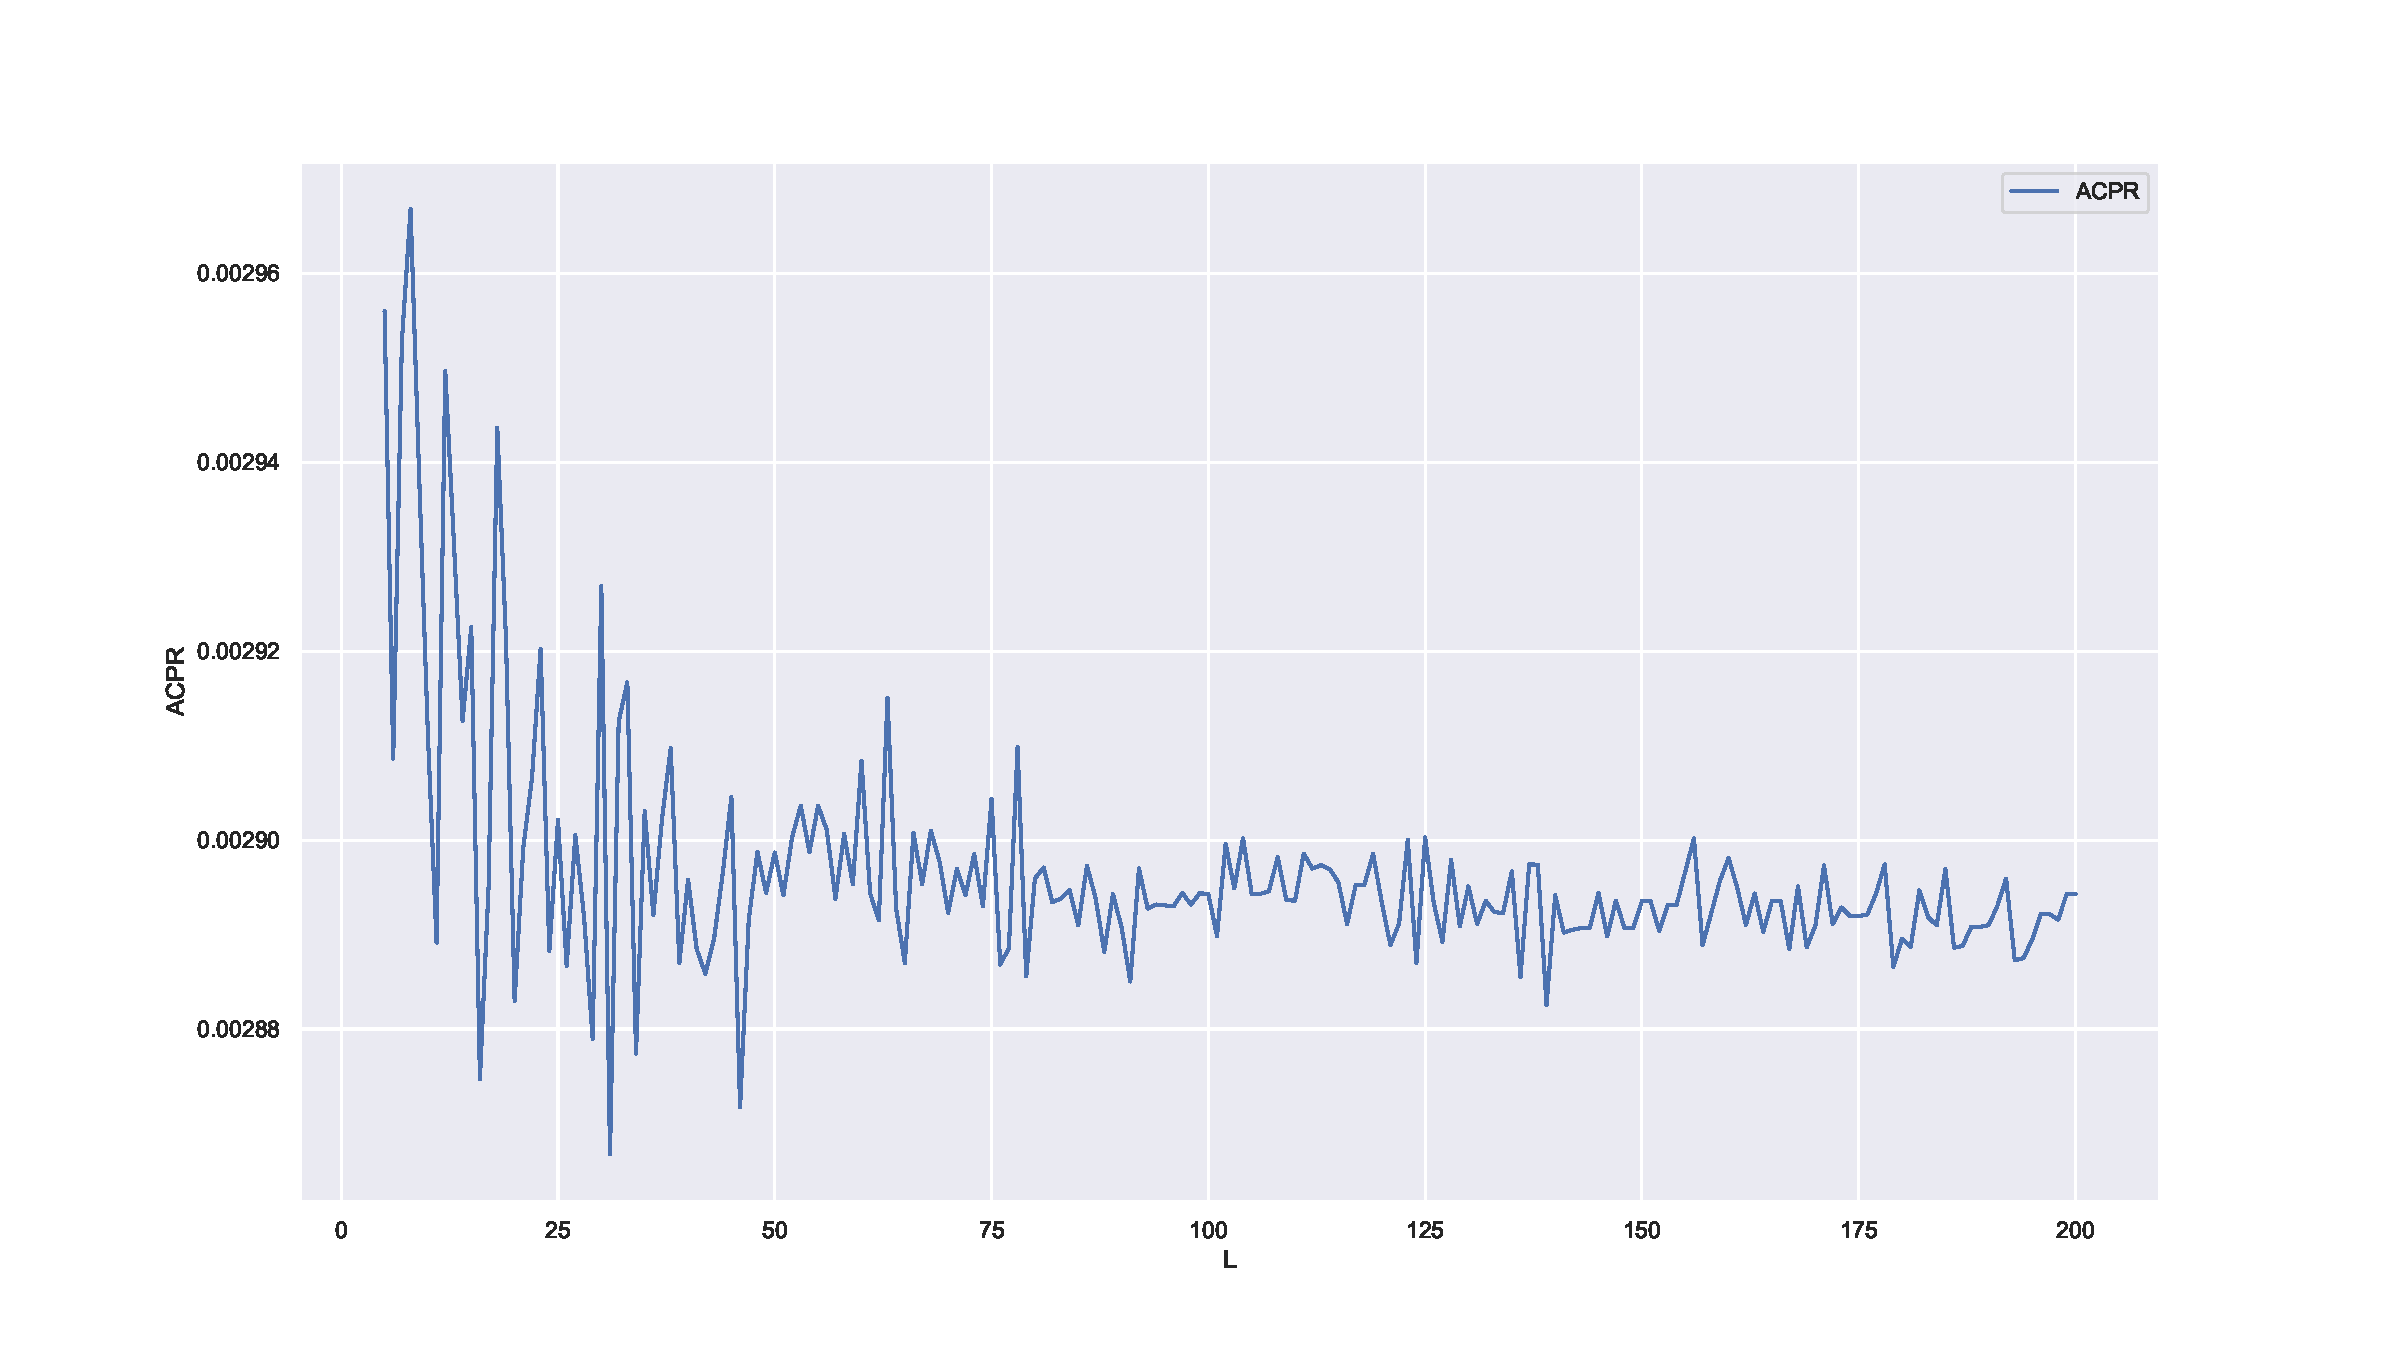
\includegraphics[width=\textwidth]{twap_acpr.pdf}
            \caption{TWAP ACPR dynamics as a function of frequency of trading. $T = 200$.}
        \end{figure}

        \begin{figure}[htbp]
            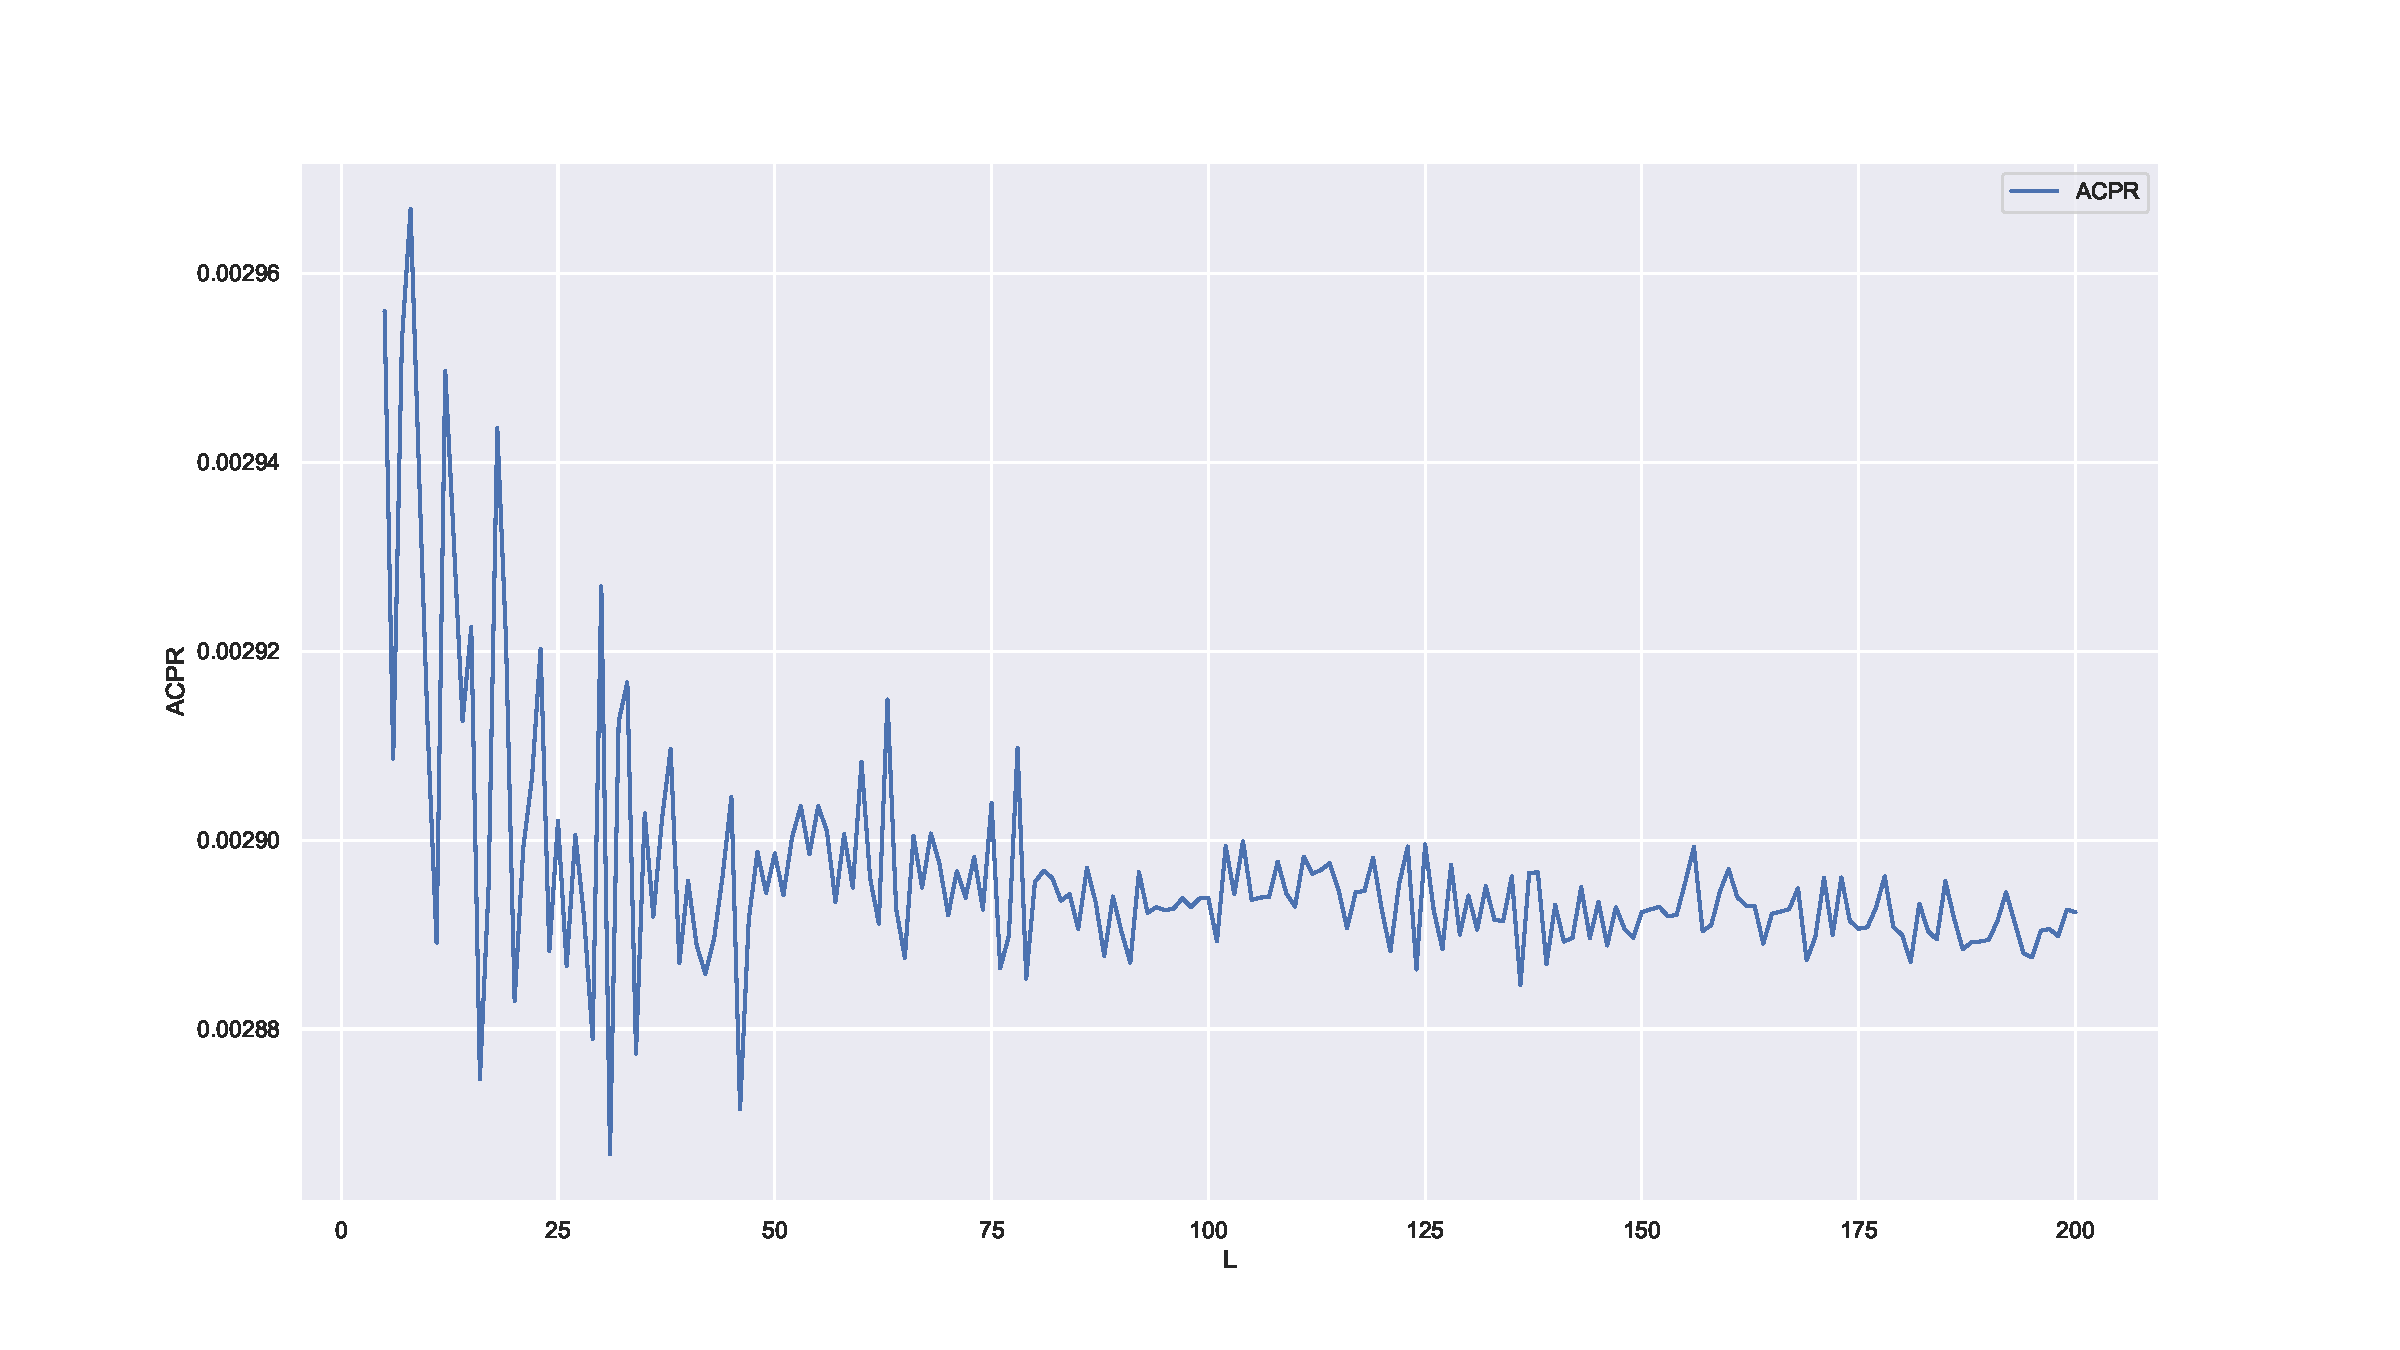
\includegraphics[width=\textwidth]{ac_acpr.pdf}
            \caption{Almgren-Chriss ACPR dynamics as a function of frequency of trading. $T = 200$.}
        \end{figure}